%%%%%%%%%%%%%%%%%%%%%%%%%%%%%%%%%%%%%%%%%%%%%%%%%%%
%% P3: Phenomenology of Particle Physics                         
%%
%% Author:  André Rubbia                   		 
%%
%% Figure 2.14 Trajectories depend on the impact parameter.
%%
%% This work is licensed under the Creative Commons Attribution 4.0 International License. 
%% To view a copy of this license, visit http://creativecommons.org/licenses/by/4.0/ or 
%% send a letter to Creative Commons, PO Box 1866, Mountain View, CA 94042, USA.
%%
%%%%%%%%%%%%%%%%%%%%%%%%%%%%%%%%%%%%%%%%%%%%%%%%%%%

\documentclass[a4paper,10pt]{article}

\usepackage[T1]{fontenc}
\usepackage[utf8]{inputenc}
\usepackage{lmodern}
\usepackage[labelfont=bf]{caption}
\usepackage{upgreek}
\usepackage{amssymb}
\usepackage{amsmath}

\usepackage{tikz}
\usepackage{pgfplots}
\pgfplotsset{compat=1.17}
\usepgfplotslibrary{ternary}
\usepgfplotslibrary{fillbetween}
\usepgfplotslibrary{external}


\def\d{\mathrm{d}}

\begin{document}

%%%%%%%%%%%%%%%   FIGURE  %%%%%%%%%%%%%%%%%%%%%%%%%%%%%%
\begin{figure}[htb]
\begin{center}
%%%\includegraphics[width=0.55\textwidth]{BasicConcepts/streuexperiment.pdf}
    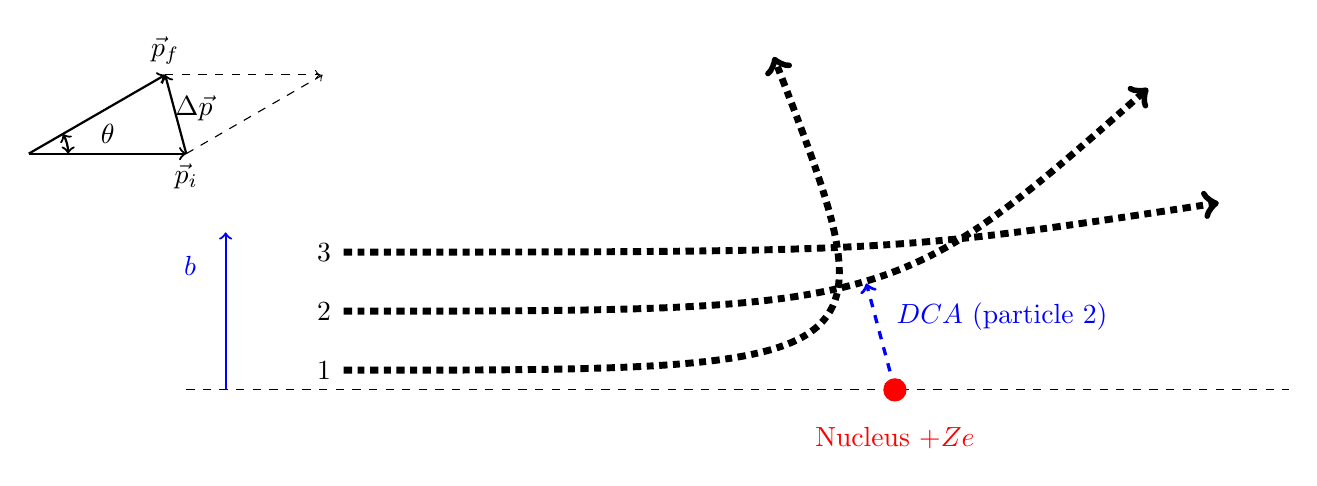
\begin{tikzpicture}[scale=1.]
         \draw[dashed] (-9,0) -- (5,0);
        \draw[line width=2.5, dash dot,->] (-7,0.25) node[left] {1} .. controls (0,0.25) .. (110:4.5);
        \draw[line width=2.5, dash dot,->] (-7,1) node[left] {2} .. controls (0,1) .. (50:5.);
        \draw[line width=2.5, dash dot,->] (-7,1.75) node[left] {3} .. controls (0,1.75) .. (30:4.75);
         \draw[<->,blue, dashed, very thick] (0,0) -- (105:1.4) node[right=7pt, yshift=-12pt] {$DCA$ (particle 2)};
         \filldraw [red] (0,0) circle (4pt) node[below=10pt] {Nucleus $+Ze$};
         \draw[thick,blue,->] (-8.5,0) -- (-8.5,2) node[left=7pt, yshift=-12pt] {$b$};

            \begin{scope}[shift={(-11,3)}]
            \draw[thick, ->] (0,0) -- (2,0) node[below] {$\vec p_i$};
            \draw[thick, ->] (0,0) -- (30:2) node[above] {$\vec p_f$};
            \draw[dashed, ->] (30:2) -- (3.7,1) ;
            \draw[dashed, ->] (2,0) -- +(30:2) ;
            \draw[thick, ->] (2,0) -- (30:2) node[right, yshift=-12pt] {$\Delta \vec  p$};
            \draw[thick,<->] (0.5,0.) arc (0:30:0.5) node[right=10pt, yshift=0pt] {$\theta$};
	   \end{scope}

  \end{tikzpicture}
\caption{Trajectories depend on the impact parameter.}
\end{center}
\end{figure}
%%%%%%%%%%%%%%%   END FIGURE  %%%%%%%%%%%%%%%%%%%%%%%%%%%%%%

\end{document}
